%! Author = eliainnocenti
%! Date = 27/12/23

% Preamble
\documentclass[11pt]{article}

% Packages
\usepackage{amsmath}
\usepackage{graphicx}
\usepackage{float}
\usepackage{listings}
\usepackage[font=small]{caption}
\usepackage{comment}
\usepackage[linesnumbered,vlined]{algorithm2e}
\usepackage{hhline}
\usepackage{geometry}
\usepackage{tabularx}

% Images path
\graphicspath{ {../out/}
             }

% Layout settings
\renewcommand{\contentsname}{Index}
\renewcommand{\figurename}{Figure}
\renewcommand{\tablename}{Table}
\SetAlgoCaptionSeparator{}
\begin{comment}
\geometry{
    bottom=2.8cm
}
\end{comment}

% Style
\lstdefinestyle{mystyle}{
    basicstyle=\ttfamily\footnotesize,
    breakatwhitespace=false,
    breaklines=true,
    captionpos=b,
    keepspaces=true,
    numbers=left,
    numbersep=5pt,
    showspaces=false,
    showstringspaces=false,
    showtabs=false,
    tabsize=2
}
\lstset{style=mystyle}

% Document intestation
\title{Simulated Annealing e TSP \\
       \vspace{0.5em}
       \large Simulated Annealing: implementazione e \\
              applicazione al problema del commesso viaggiatore}
\author{Elia Innocenti}
\date{Gennaio 2024}

% Document
\begin{document}

    \newgeometry{top=1.7cm, bottom=2.8cm}

    \maketitle

    % Introduction
    \section{Introduzione} \label{sec:introduction}

        Questa relazione descrive il lavoro svolto per l'esercizio assegnato di Intelligenza Artificiale.
        L'assegnazione prevede: di implementare l'algoritmo di Simulated Annealing (nella semplice versione descritta in R&N 2009 §4.1.2) e
        di applicarlo al problema del commesso viaggiatore (Travelling Salesman Problem),
        ovvero della ricerca di un ciclo di costo minimo che copre tutti i vertici di un grafo assegnato.
        Viene fornito inoltre un esempio di applicazione classica del Simulated Annealing (V. Černý, 1985).

    % Algorithm analysis
    \section{Analisi dell'algoritmo} \label{sec:algorithm_analysis}

        La versione dell'algorimo a cui si fa riferimento è quello riportato in R&N 2009 §4.1.2.

        \SetAlgorithmName{}{simulated_annealing}{}
        \begin{algorithm}[H] \label{alg:simulated_annealing_algorithm}
            \SetAlgoLined
            \vspace{0.5em}
            \captionabove{\underline{SIMULATED-ANNEALING(problema, velocità\_raffreddamento)}} \\
            \vspace{0.5em}

                $corrente$ \leftarrow $problema.STATOINIZIALE$ \\
                \For{$t \leftarrow 1$ \KwTo \inf}{
                    $T$ \leftarrow $velocità\_raffreddamento[t]$ \\
                    \If{$T = 0$}{
                        \Return $corrente$
                    }
                    $successivo$ \leftarrow \textnormal{ un successore a caso di} $ corrente$ \\
                    $\Delta E$ \leftarrow $VALORE(corrente) - VALORE(successivo)$ \\
                    \If{$\Delta E > 0$}{
                        $corrente$ \leftarrow $successivo$ \\
                    }
                    \Else {
                        $corrente$ \leftarrow $successivo $ \textnormal{con probabilità} $ e^{\Delta E/T}$ \\
                    }
                }
        \end{algorithm}

    \restoregeometry



    % Implementation
    \section{Implementazione} \label{sec:implementation}

        L'algoritmo è stato implementato in python, riceve in input il problema e il cooling rate (velocità di raffreddamento).
        Si è voluta mantenere una struttura quanto più fedele allo pseudocodice fornito dal R&N 2009, di conseguenza la permutazione delle stazioni e
        la generazione dei nuovi path è affidata ad un metodo del problema (implementato come classe).
        L'algoritmo utilizza il metodo $get\_initial\_state()$ per ricevere lo stato iniziale, $get\_random\_successor()$ per ricevere un
        successore dello stato iniziale (un random path generato a partire dallo stato corrente) e le funzioni di valutazione $calculate\_value()$
        per valutare gli stati (calcola quindi la lunghezza dei path).
        Per la modellizzazione del problema è stato seguito il paper: viene utilizzata una matrice di incidenza $D$ i cui elementi $D(i,j)$ rappresenzano il
        peso dell'arco che va dal nodo $i$ al nodo $j$; i nodi sono invece numerati con degli interi che vanno da $0$ a $N-1$, dove $N$ è la dimensione della matrice.
        Il cooling rate è implementabile in vari modi, in questo caso viene costruito un array di dimensione max\_iteration con i valori della temperatura che
        segue un certo andamento.

    % Test and results
    \section{Test e risultati} \label{sec:test_and_results}

        È stato effettuato un test per il funzionamento con una matrice (file matrix1.py): dimensione $10*10$ (le stazioni sono quindi $10$) e
        contiene valori che vanno da $0$ a $10$.

        \begin{figure}[h]
            \centering
            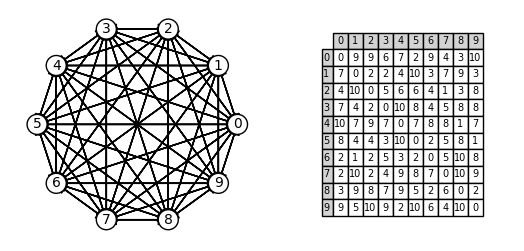
\includegraphics[width=0.8\textwidth]{matrix1}
            \caption{matrice di incidenza del problema e grafo associato.}
            \label{fig:matrix1}
        \end{figure}

        In questo test, è stato verificato che con un tipo di cooling rate esponenziale (con alpa = 0.7), una temperatura iniziale = 10000,
        un numero massimo di iterazioni = 100 e un numero di trials = 1000, si trova sempre il percorso di costo minimo.
        Il costo computazionale (il numero di iterazioni e di trials) è di molto migliorabile se si studia più approfonditamente il modello
        del problema specifico in questione per ottenere dei paramtri più efficaci.

    % Conclusion
    \section{Conclusioni} \label{sec:conclusiona}

        Come anche specificato nella ricerca, l'algoritmo riesce sempre a stimare il cammino ciclico di costo minimo dato un certo numero di trials,
        e spesso a trovarlo in maniera esatta. \\
        Viene inoltre specificato che la correttezza dell'algoritmo non è dimostrata con teoremi rigorosi, ma il funzionamento di
        questo viene comunque mostrato e supportato grazie ad un'ampia serie di esempi (vedesi il paper). \\
        C'è da dire anche che le esecuzioni dell'algoritmo per uno specifico problema sono sempre migliorabili se viene fatto uno studio approfondito
        sui parametri che caratterizzano la modellazione del problema stesso. Infatti se si agisce sulla velocità di raffreddamento, sulla temperatura iniziale,
        sul numero massimo di iterazioni, e così via, si possono ottenere risultati molto diversi. È vero anche che, se si utilizzano dei parametri che
        funzionano per un determinato problema, non è detto che funzionino per un problema diverso, proprio per questo è importante studiare ù
        la modellizzazione del problema ed effettuare un numero sufficiente di test.

    % Bibliography
    \section{Bibliografia} \label{sec:bibliography}

        \begin{enumerate}
            \item Russell, S., & Norvig, P. (2009). Artificial Intelligence: A Modern Approach (3rd ed.)
            \item Thermodynamical Approach to the Traveling Salesman Problem: An Efficient Simulation Algorithm, V. Černý, 1985
        \end{enumerate}

\end{document}